\section{Đánh giá hệ thống}
\noindent Hệ thống sử dụng Apache Kafka trên Confluent Cloud để thực hiện thu thập dữ liệu thời gian thực từ các thiết bị tài sản công nghệ thông tin, bao gồm phần cứng và phần mềm. Thành phần Kafka Producer được triển khai trên các thiết bị đầu cuối để đẩy dữ liệu lên Kafka Cluster, trong đó mỗi sự kiện hoặc thông tin liên quan đến tài sản (như trạng thái hoạt động, lỗi phát sinh, hiệu năng) được gửi dưới dạng thông điệp (message). \\ \\
Kafka Producer: Gửi thông điệp từ các thiết bị IT Users lên Kafka Cluster.
Kafka Broker: Tiếp nhận và lưu trữ tạm thời thông điệp, chờ các dịch vụ tiêu thụ.
Consumer: Các thành phần như Asset Monitoring Service và Alert \& Notification Service tiêu thụ dữ liệu để thực hiện phân tích và đưa ra các cảnh báo.
\subsection{Đánh giá hiệu năng thu thập dữ liệu thời gian thực với Kafka}
\noindent Đánh giá hiệu năng Kafka qua \textit{kafka-producer-perf-test} và \textit{kafka-consumer-perf-test} mà Kafka hỗ trợ.\\ \\
Với mục tiêu đề tài là thiết kế hệ thống cho đối tượng công ty vừa và nhỏ, với số lượng máy tính nằm trong khoảng 50 - 100, nhóm đã thực hiện đánh giá qua giả lập như sau (bỏ qua độ trễ của môi trường mạng):
\begin{enumerate}
    \item \textbf{Producer}\\
        \textbf{Mục tiêu}: Đánh giá hiệu năng của Kafka Producer dựa trên các chỉ số tốc độ gửi (MB/sec), độ trễ trung bình (ms) và độ trễ lớn nhất (ms) với các kích thước gói tin và số lượng máy tính khác nhau.\\
        Phương pháp: 
        \begin{longtable}{|p{0.1\textwidth}|p{0.12\textwidth}|p{0.2\textwidth}|p{0.2\textwidth}|p{0.2\textwidth}|}
            \caption{Đánh giá Producer}\\
            \hline
            \textbf{Số lượng máy tính} & \textbf{Kích thước gói tin (byte)} & \textbf{Tốc độ gửi (MB.sec)} & \textbf{Độ trễ trung bình (ms)} & \textbf{Độ trễ lớn nhất (ms)} \\
            \hline
            5 & 20000 & 0.27 & 75 & 302\\
            \hline
            25 & 20000 & 1.41 & 46.96 & 301\\
            \hline
            50 & 20000 & 1.78 & 54.78 & 308\\
            \hline
            75 & 20000 & 3.41 & 59.31 & 346\\
            \hline
            100 & 20000 & 4.7 & 68.76 & 425\\
            \hline
            125 & 20000 & 5.51 & 69.17 & 453\\
            \hline
             5 & 50000 & 0.35 & 93 & 313\\
            \hline
            25 & 50000 & 1.41 & 46.96 & 301\\
            \hline
            50 & 50000 & 3.52 & 45 & 298\\
            \hline
            100 & 50000 & 11.66 & 48.05 & 330\\
            \hline
            125 & 50000 & 14.33 & 65.67 & 332\\
            \hline
        \end{longtable}
        \begin{itemize}[label=--]
            \item  Ảnh hưởng của số lượng máy tính: Nhìn chung, tốc độ gửi tăng khi số lượng máy tính, mỗi máy tính tương ứng với một gói tin. Điều này cho thấy Producer có khả năng xử lý hiệu quả lượng lớn tin nhắn. Tuy nhiên, độ trễ trung bình và độ trễ lớn nhất cũng có xu hướng tăng, đặc biệt khi số lượng record vượt quá 100.
            \item Ảnh hưởng của kích thước gói tin: Khi tăng kích thước gói tin từ 20000 byte lên 50000 byte (với 50 record), tốc độ gửi tăng đáng kể (từ 1.78 MB/sec lên 3.52 MB/sec) trong khi độ trễ trung bình giảm. Điều này cho thấy Producer có thể xử lý các record lớn một cách hiệu quả.
            \item Độ trễ: Độ trễ trung bình dao động trong khoảng 45 ms đến 93 ms, cho thấy Producer gửi tin nhắn với độ trễ tương đối thấp. Tuy nhiên, độ trễ lớn nhất có thể lên đến 453 ms, cho thấy có sự không đồng đều về độ trễ giữa các tin nhắn.
        \end{itemize}
        => \textbf{Kafka Producer} cho thấy hiệu năng tốt với khả năng xử lý lượng lớn tin nhắn và các record có kích thước lớn. Tuy nhiên, cần lưu ý đến sự gia tăng độ trễ khi số lượng record tăng cao.
    \item \textbf{Consumer}\\
        \textbf{Mục tiêu}: Đánh giá hiệu năng của Kafka Consumer dựa trên các chỉ số tốc độ tiêu thụ (MB/sec), độ trễ (ms) và thời gian rebalance (ms) với số lượng message khác nhau.
    
        \begin{longtable}{|p{0.2\textwidth}|p{0.2\textwidth}|p{0.2\textwidth}|p{0.3\textwidth}|}
        \caption{Đánh giá Consumer}\\
        \hline
        \textbf{Số lượng gói tin} & \textbf{Tốc độ tiêu thụ (MB.sec)} & \textbf{Độ trễ (ms)} & \textbf{Thời gian Rebalance (ms)}  \\
        \hline
        5 & 2.709 & 47 & 314\\
        \hline
        50 & 2.665 & 46 & 316\\
        \hline
        75 & 2.775 & 47 & 319\\
        \hline
        100 & 2.802 & 46 & 321\\
        \hline
        125 & 2.685 & 47 & 321\\
        \hline
    \end{longtable}
    \begin{itemize}[label=--]
            \item Tốc độ tiêu thụ: Tốc độ tiêu thụ dữ liệu dao động trong khoảng 2.665 MB/sec đến 2.802 MB/sec. Không có sự thay đổi đáng kể về tốc độ tiêu thụ khi số lượng message tăng. Điều này cho thấy Consumer duy trì hiệu năng ổn định khi xử lý lượng message khác nhau.
            \item Độ trễ: Độ trễ trung bình dao động quanh mức 46-47 ms, cho thấy Consumer có thể nhận và xử lý tin nhắn một cách nhanh chóng.
            \item Thời gian rebalance: Thời gian trung bình dành cho rebalance (ms). Rebalance thường xuyên và mất nhiều thời gian có thể ảnh hưởng đáng kể đến hiệu năng của consumer. Thời gian rebalance dao động trong khoảng 314 ms đến 321 ms. Mặc dù thời gian rebalance không quá cao, nhưng rebalance thường xuyên có thể ảnh hưởng đến hiệu năng tổng thể của Consumer.
        \end{itemize}
        => \textbf{Kafka Consumer} thể hiện hiệu năng ổn định với tốc độ tiêu thụ dữ liệu và độ trễ thấp. Tuy nhiên, cần theo dõi thời gian rebalance để đảm bảo nó không gây ảnh hưởng đáng kể đến hiệu năng.
\end{enumerate} 
\subsection{Đánh giá hiệu năng Confluent Cloud trong quá trình thu thập dữ liệu}
\noindent Để đánh giá hiệu năng của hệ thống truyền tải dữ liệu sử dụng nền tảng \textbf{Confluent Kafka}, nhóm đã tiến hành kiểm thử với nhiều mức tải khác nhau (số lượng messages từ 25 đến 200) và phân tích các chỉ số quan trọng bao gồm: Throughput (Thông lượng), Latency (Độ trễ) và mối quan hệ giữa hai yếu tố này. 
Bảng kết quả thực nghiệm như sau:
\begin{longtable}{|p{0.1\textwidth}|p{0.12\textwidth}|p{0.2\textwidth}|p{0.2\textwidth}|p{0.2\textwidth}|}
    \caption{Kết quả thực nghiệm}\\
    \hline
    \textbf{Số lượng máy tính}  & \textbf{Tốc độ gửi (MB/s)} & \textbf{Độ trễ trung bình (ms)} & \textbf{Độ trễ lớn nhất (ms)} & \textbf{Độ trễ nhỏ nhất (ms)} \\
    \hline
    20  & 14.18 & 1181.93 & 1305.33 & 1113.18 \\
    \hline
    50  & 30.31 & 1170.77 & 1260.23 & 1106.45 \\
    \hline
    75  & 44.26 & 1155.42 & 1227.83 & 1086.95 \\
    \hline
    100 & 48.41 & 1170.30 & 1294.78 & 1090.63 \\
    \hline
    125 & 57.85 & 1171.65 & 1338.35 & 1073.85 \\
    \hline
    150 & 63.91 & 1149.21 & 1233.85 & 1064.48 \\
    \hline
    175 & 65.23 & 1164.11 & 1322.62 & 1056.69 \\
    \hline
    200 & 71.67 & 1156.05 & 1266.38 & 1063.86 \\
    \hline
\end{longtable}
\textbf{Kết quả được trình bày qua bốn biểu đồ chính như sau}:
\begin{figure}[H]
    \centering
    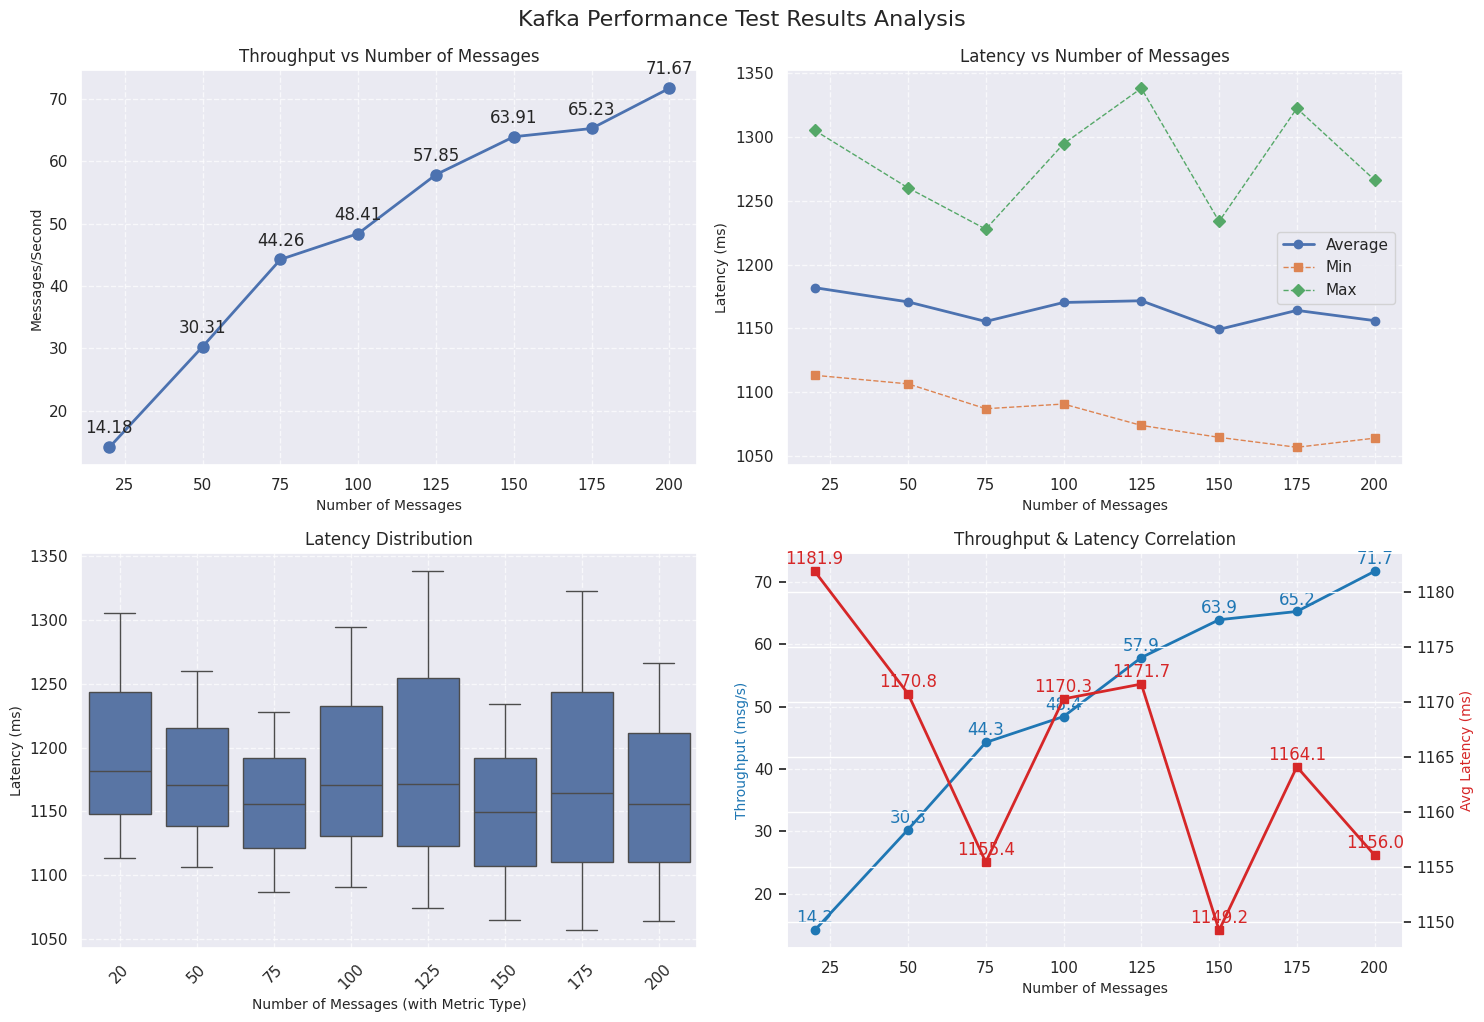
\includegraphics[width=\linewidth]{Images//C7/testchart.png}
    \vspace{10pt}
    \caption{Biểu đồ đánh giá hiệu năng Kafka trên Confluent Cloud}
    \label{fig:enter-label}
\end{figure}
\textbf{Nhận xét}:
\begin{itemize}[label=--]
    \item \textbf{Thông lượng và số lượng tin nhắn}: thông lượng tăng ổn định theo số lượng messages gửi vào, từ 14.18 msg/s (25 messages) lên đến 71.67 msg/s (200 messages). Biểu đồ thể hiện hiệu suất hệ thống được mở rộng tốt với tải tăng dần, phản ánh khả năng scalability (mở rộng) của Kafka và Confluent Cloud. Tuy nhiên, tốc độ tăng throughput chậm lại sau mốc 125 messages, cho thấy điểm tiệm cận của hiệu suất hoặc giới hạn băng thông/partition.
    \item \textbf{Độ trễ và số lượng tin nhắn}: Độ trễ trung bình duy trì ổn định trong khoảng 1150–1200 ms, ngay cả khi số lượng messages tăng lên. Độ trễ nhỏ nhất giảm dần từ ~1125 ms xuống còn khoảng 1080 ms, cho thấy hiệu quả xử lý được cải thiện với khối lượng tải cao hơn. Độ trễ lớn nhất dao động mạnh (từ 1250 ms đến hơn 1300 ms), phản ánh rằng vẫn tồn tại những đỉnh tải (latency spike) có thể ảnh hưởng đến trải nghiệm thời gian thực nếu không được tối ưu.
    \item \textbf{Phân phối độ trễ}: Phân phối độ trễ tương đối đều trong từng mức tải, với độ lệch chuẩn vừa phải. Một số mức tải (125, 175) có dải phân bố latency rộng hơn, chứng tỏ có dao động nhất định trong hiệu suất khi hệ thống xử lý khối lượng dữ liệu lớn hơn. Không có trường hợp cực đoan (outlier nghiêm trọng), thể hiện hệ thống tương đối ổn định và đáng tin cậy.
    \item \textbf{Mối tương quan giữa Thông lượng và Độ trễ}: Biểu đồ này cho thấy khi throughput tăng, độ trễ trung bình không tăng theo, ngược lại còn giảm nhẹ từ ~1181 ms xuống ~1156 ms. Điều này phản ánh rằng Kafka hoạt động hiệu quả hơn dưới tải cao, nhờ vào cơ chế batch và xử lý bất đồng bộ của nó. Không có dấu hiệu nghẽn cổ chai khi throughput tăng — một kết quả rất tích cực cho việc mở rộng hệ thống theo chiều ngang.
\end{itemize}
=> \textbf{Kết luận}: Kết quả này xác nhận Kafka trên Confluent Cloud là giải pháp phù hợp cho các hệ thống cần xử lý luồng dữ liệu ổn định ở quy mô vừa, với tiềm năng mở rộng tuyến tính khi tăng số partitions. Độ trễ ổn định và không có outlier cực đoan là điểm mạnh nổi bật, đảm bảo độ tin cậy cho các ứng dụng nghiệp vụ quan trọng.
\subsection{Đánh giá hiệu năng thu thập dữ liệu phần cứng và phần mềm}
\noindent Nhóm đã tiến hành phát triển công cụ Collector để thu thập dữ liệu phần cứng và phần mềm. Collector được thiết kế như là một producer của Kafka. Collector được xây dựng dựa trên ngôn ngữ Python.\\ \\
Nhóm sẽ đánh giá Collector qua các tiêu chí như sau : Hiệu năng, độ chính xác và toàn vẹn dữ liệu, mức độ thân thiện.
\begin{enumerate}
    \item \textbf{Hiệu năng}\\
    Nhóm đã tiến hành chạy Collector với kết quả như sau:
    \begin{itemize}[label=--]
        \item Thời gian thực thi:
        Nhóm sử dụng thư viện Time của Python để tiến hành đánh giá qua 10 lần chạy thử và kết quả đạt được như sau :
        \begin{itemize}[label=\textbullet]
            \item Thời gian thực thi nhanh nhất: 3.2 s
            \item Thời gian thực thi chậm nhất: 3.6075 s
            \item Thời gian thực thi trung bình: 3.41 s
        \end{itemize}
        => Điều này cho thấy thời gian thực thi của công cụ khá ổn định, không có sự dao động lớn giữa các lần chạy. Các yếu tố ảnh hưởng nhỏ như tải của hệ thống hoặc môi trường thực thi có thể là nguyên nhân chính cho sự dao động này. Thời gian quét này khá phù hợp để tích hợp trong hệ thống IT asset management mà không gây gián đoạn hoạt động.

        \item Sử dụng tài nguyên hệ thống:\\
        Nhóm tiến hành đo dựa trên mức sử dụng CPU và RAM của tiến trình thực thi quét. Kết quả sau 10 lần chạy cho thấy:
        \begin{itemize}[label=\textbullet]
            \item RAM dao động từ 33MB đến 34MB là rất nhỏ và cho thấy công cụ Scanner sử dụng tài nguyên bộ nhớ một cách hiệu quả. Biên độ dao động 1MB cho thấy sự ổn định trong việc quản lý bộ nhớ, không có dấu hiệu rò rỉ bộ nhớ (memory leak).
            \item CPU dao động từ 0.00\% đến 0.1\%. Điều này thể hiện rằng công cụ Collector không chiếm dụng tài nguyên CPU đáng kể trong quá trình quét.
        \end{itemize}
    \end{itemize}
    \item \textbf{Mức độ thân thiện}
    \begin{itemize}[label=--]
        \item Collector được thiết kế để chạy ngầm trên máy mà không ảnh hưởng đến nhân viên khi sử dụng máy tính để bàn và laptop cá nhân.  
        \item Nhân viên IT có thể dễ dàng cài đặt công cụ Collector trên tài sản máy tính mới.
        \item Tuy nhiên, Collector mới chỉ có khả năng cài đặt trên môi trường Window với phiên bản tối thiểu là Windows 7.
        \item Quy trình chạy Collector đơn giản, nhân viên IT chỉ cần bấm nút chạy và cài đặt cho chương trình khởi động cùng máy là có thể vận hành.
    \end{itemize}
    => Collector được thiết kế thân thiện với người dùng nhưng chưa có khả năng tương thích với đa nền tảng. 
    \\ Quy trình vận hành đơn giản nhằm đơn giản hóa các quy trình cho hệ thống. 
    \item \textbf{Toàn vẹn dữ liệu}\\
     Các trường hợp ảnh hưởng đến khả năng toàn vẹn dữ liệu:
        \begin{itemize}[label=--]
            \item Server Kafka sập: thông tin từ Collector sẽ không đến được Kafka Server.
            \item Lỗi hệ thống: hệ điều hành quá cũ hoặc không tương thích với hệ điều hành sẽ khiến cho dữ liệu bị thiếu mất hoặc không thu thập được
            \item Tắc nghẽn mạng: tình trạng mạng tắc nghẽn sẽ làm gói tin mà Producer gửi đến Kafka Server chậm, làm mất đi độ chính xác về thời gian.
        \end{itemize}
\end{enumerate}

\subsection{Đánh giá hiệu suất hệ thống}
\subsubsection{Giới thiệu công cụ và chỉ số đánh giá}
\noindent Để đánh giá hiệu năng hệ thống, nhóm sử dụng công cụ mã nguồn mở \textbf{K6} \cite{k6} – một nền tảng kiểm thử hiệu suất hiện đại được thiết kế để kiểm tra khả năng chịu tải của hệ thống backend. K6 hỗ trợ viết kịch bản bằng JavaScript, có thể mô phỏng hàng nghìn người dùng ảo (VUs – Virtual Users) thực hiện các hành động giống người dùng thật.
\begin{figure}[H]
    \centering
    
\includegraphics[width=0.5\linewidth]{Images/C7/k6.png}
    \vspace{15pt}
    \caption{K6\\ Nguồn: k6.io, truy cập vào ngày 01/05/2025}
\end{figure}
\noindent Các chỉ số quan trọng được đo trong quá trình đánh giá:
\begin{itemize}[label=--]
    \item \textbf{HTTP request duration (http\_req\_duration)}: Thời gian từ khi gửi request đến khi nhận toàn bộ phản hồi từ máy chủ.
    \item \textbf{Response time percentiles (p90, p95)}: Phân vị thống kê thời gian phản hồi – ví dụ, \textit{p90} nghĩa là 90\% request có thời gian phản hồi thấp hơn giá trị này.
    \item \textbf{Checks}: Tỉ lệ các điều kiện được kiểm tra (ví dụ mã phản hồi 200 hoặc thời gian phản hồi < 2000ms) đạt yêu cầu.
    \item \textbf{Http request failed (http\_req\_failed)}: Tỉ lệ request bị lỗi (timeout, lỗi mạng, hoặc lỗi server).
    \item \textbf{VUs và VUs max}: Số người dùng ảo đồng thời đang chạy và giá trị cực đại theo cấu hình.
\end{itemize}
\noindent Các chỉ số này giúp đánh giá toàn diện khả năng phản hồi và mức độ ổn định của hệ thống trong điều kiện tải thực tế và cực đại.

\subsubsection{Đánh giá hiệu suất}
\noindent Để kiểm tra khả năng chịu tải và hiệu suất phản hồi của hệ thống quản lý tài sản CNTT (ITAM), nhóm đã tiến hành kiểm thử hiệu năng sử dụng K6. Kịch bản kiểm thử được thiết kế mô phỏng 200 người dùng ảo (Virtual Users - VUs) truy cập đồng thời vào các API cốt lõi trong vòng 60 giây, lặp lại nhiều lần để thu thập dữ liệu ổn định.
\subsubsection*{1. Danh mục API đánh giá}
\begin{table}[H]
    \centering
    \caption{Các API cần test hiệu suất theo mục tiêu}
    \begin{tabular}{|>{\raggedright\arraybackslash}p{6cm}|>{\raggedright\arraybackslash}p{8cm}|}
        \hline
        \textbf{Mục tiêu chính} & \textbf{API liên quan nên test hiệu suất} \\
        \hline
        Dashboard \& Tổng quan (thường tải mỗi lần đăng nhập) & 
        \texttt{GET /api/dashboard}\newline
        \texttt{GET /api/overview/computer}\newline
        \texttt{GET /api/overview/software}\newline
        \texttt{GET /api/overview/hardware} \\
        \hline
        Tải danh sách tài sản (asset) & 
        \texttt{GET /api/asset}\newline
        \texttt{GET /api/computer/GetComputers}\newline
        \texttt{GET /api/Software} \\
        \hline
        Giám sát hiệu suất \& cảnh báo & 
        \texttt{GET /api/performance/\{assetId\}/\{topic\}}\newline
        \texttt{GET /api/alert}\newline
        \texttt{GET /api/alert/computer/\{computerId\}} \\
        \hline
        Thêm mới / cập nhật asset hoặc alert & 
        \texttt{POST /api/asset}\newline
        \texttt{POST /api/alert}\newline
        \texttt{PUT /api/computer/UpdateComputer/\{id\}} \\
        \hline
        Đăng nhập / xác thực & 
        \texttt{POST /api/login}\newline
        \texttt{GET /api/current-user}\newline
        \texttt{POST /api/refresh-token} \\
        \hline
        Kafka / gửi dữ liệu từ agent & 
        \texttt{POST /api/kafka/firstScan}\newline
        \texttt{POST /api/kafka/upgrade} \\
        \hline
        Dự đoán hiệu suất & 
        \texttt{GET /api/performance/predict}\newline
        \texttt{POST /api/performance/predict/test} \\
        \hline
    \end{tabular}
    
\end{table}

\subsubsection*{2. Tiêu chuẩn đánh giá}
\begin{itemize}[label=--]
\item Mã trạng thái HTTP: \textbf{200} (thành công)
\item Thời gian phản hồi: \textbf{< 2000ms}
\item Không có lỗi kết nối hoặc xử lý TLS
\end{itemize}

\subsubsection*{3. Chi tiết kết quả theo nhóm API}
\begin{table}[H]
\centering
\caption{Kết quả đánh giá hiệu năng Dashboard API}
\begin{tabular}{|>{\raggedright\arraybackslash}p{4cm}|l|>{\raggedright\arraybackslash}p{7cm}|}
\hline
\multicolumn{1}{|c|}{\textbf{Chỉ số đánh giá}} & \textbf{Giá trị} & \multicolumn{1}{c|}{\textbf{Phân tích}} \\
\hline
\textbf{Tỷ lệ thành công HTTP 200} & 100\% (22800/22800) & Tất cả các yêu cầu đều được xử lý thành công, không có lỗi phản hồi từ máy chủ \\
\hline
\textbf{Thời gian phản hồi trung bình} & 61.76ms & Hệ thống phản hồi rất nhanh, chỉ mất khoảng 62ms để xử lý mỗi request — nhanh hơn nhiều so với ngưỡng tiêu chuẩn 2000ms \\
\hline
\textbf{Phân vị 90 (P90)} & 87.19ms & 90\% số request có thời gian phản hồi dưới 87.19ms, cho thấy sự ổn định rất cao về hiệu suất \\
\hline
\textbf{Phân vị 95 (P95)} & 461.91ms & 95\% request phản hồi dưới 500ms, một tỷ lệ chấp nhận được trong môi trường sản phẩm thực tế \\
\hline
\textbf{Thời gian phản hồi nhanh nhất} & 0.31ms & Phản hồi cực nhanh ở điều kiện lý tưởng, cho thấy không có độ trễ từ phía máy chủ \\
\hline
\textbf{Thời gian phản hồi chậm nhất} & 1.77s & Dù một số trường hợp phản hồi chậm, nhưng vẫn trong mức cho phép (<2s), không ảnh hưởng nhiều đến trải nghiệm người dùng \\
\hline
\textbf{Tỷ lệ lỗi} & 0\% & Không có lỗi phát sinh trong toàn bộ quá trình kiểm thử, cho thấy độ ổn định cao \\
\hline
\textbf{Lưu lượng request} & 186.68 req/s & Hệ thống xử lý trung bình gần 187 request mỗi giây, duy trì được hiệu năng ổn định dưới tải \\
\hline
\textbf{User ảo (VUs)} & 21--200 & Số lượng người dùng mô phỏng thay đổi theo kịch bản kiểm thử, giúp đánh giá khả năng mở rộng của hệ thống \\
\hline
\end{tabular}

\end{table}

\begin{table}[H]
\centering
\caption{Kết quả đánh giá hiệu năng Asset API}
\begin{tabular}{|>{\raggedright\arraybackslash}p{4cm}|l|>{\raggedright\arraybackslash}p{7cm}|}
\hline
\textbf{Chỉ số đánh giá} & \textbf{Giá trị} & \textbf{Phân tích} \\
\hline
\textbf{Tỷ lệ thành công HTTP 200} & 100\% (22800/22800) & Tất cả các request đến các API chính đều được xử lý thành công, không có lỗi xảy ra \\
\hline
\textbf{Thời gian phản hồi trung bình} & 78.38ms & Phản hồi trung bình rất tốt, thấp hơn nhiều so với ngưỡng khuyến nghị 2000ms \\
\hline
\textbf{Phân vị 90 (P90)} & 218.72ms & 90\% request có phản hồi dưới 219ms, hiệu suất ổn định và đáng tin cậy \\
\hline
\textbf{Phân vị 95 (P95)} & 514.24ms & 95\% request phản hồi dưới 515ms, phù hợp cho môi trường thực tế \\
\hline
\textbf{Phản hồi nhanh nhất} & 0ms & Một số request được phản hồi gần như tức thì, không có độ trễ đáng kể \\
\hline
\textbf{Phản hồi chậm nhất} & 666.43ms & Request chậm nhất vẫn dưới 1s, đảm bảo không gây ảnh hưởng lớn đến trải nghiệm người dùng \\
\hline
\textbf{Tỷ lệ lỗi} & 0\% & Không có lỗi hệ thống nào phát sinh trong toàn bộ quá trình\\
\hline
\textbf{Lưu lượng request} & (181.87 req/s) & Hệ thống xử lý gần 182 yêu cầu mỗi giây, hiệu năng cao dưới tải vừa phải \\
\hline
\textbf{User ảo (VUs)} & 40--200 & Số lượng user mô phỏng tăng dần để kiểm tra khả năng chịu tải theo thời gian \\
\hline
\end{tabular}
\end{table}

\subsubsection*{Nhận xét tổng quan:}
\begin{itemize}[label=--]
\item Tất cả các API được đánh giá đều hoạt động ổn định với:
\begin{itemize}[label=\textbullet]
\item \textbf{Tỷ lệ thành công 100\%}, không có lỗi hệ thống trong suốt quá trình kiểm thử (tổng cộng 22,800 request)
\item \textbf{Thời gian phản hồi trung bình thấp}, dao động trong khoảng 62ms đến 78ms — thấp hơn rất nhiều so với ngưỡng tiêu chuẩn 2000ms
\item \textbf{Phân vị P90 và P95} đều nằm trong khoảng dưới 220ms và 515ms, phản ánh hiệu suất nhất quán và độ trễ thấp
\item \textbf{Lưu lượng xử lý cao} với trung bình khoảng 182 request mỗi giây, cho thấy hệ thống đủ khả năng phục vụ đồng thời nhiều người dùng
\item \textbf{Không có request thất bại}, chứng minh tính ổn định và đáng tin cậy của hệ thống trong điều kiện tải trung bình đến cao
\end{itemize}
\item Với kết quả này, hệ thống có thể hoạt động với hiệu năng ổn định ở tải vừa, sẵn sàng đưa vào vận hành thực tế. Tuy nhiên với dữ liệu lớn hơn cần kiểm thử và tối ưu thêm về mặt hiệu năng.
\end{itemize}

\subsubsection{Yêu cầu chức năng}
\begin{table}[H]
    \centering
    \caption{Checklist đánh giá yêu cầu chức năng}
    \begin{tabular}{|l|l|l|}
        \hline
        \textbf{Yêu cầu chức năng} & \textbf{Nhóm người dùng} & \textbf{Yes/No} \\
        \hline
        Giám sát tài sản & Nhân viên IT & Yes \\
        \hline
        Quản lý vòng đời tài sản & Quản lý, Nhân viên IT & Yes \\
        \hline
        Quản lý dữ liệu phần cứng và phần mềm & Nhân viên IT & Yes \\
        \hline
        Quản lý tài chính & Quản lý & Yes \\
        \hline
        Quản lý đơn đặt hàng & Quản lý & Yes \\
        \hline
        Cảnh báo và thông báo & Nhân viên IT & Yes \\
        \hline
        Tích hợp với các hệ thống khác & Quản trị viên hệ thống & No \\
        \hline
        Theo dõi hợp đồng bảo trì & Quản lý, Nhân viên IT & Yes \\
        \hline
        Quản lý giấy phép phần mềm & Quản lý, Nhân viên IT & Yes \\
        \hline
        Quản lý tuân thủ quy định & Quản lý & No \\
        \hline
        Báo cáo và phân tích & Quản lý & Yes \\
        \hline
        Quản lý sự cố và bảo trì tài sản & Nhân viên IT & Yes \\
        \hline
        Theo dõi thông tin địa điểm tài sản & Nhân viên IT & Yes \\
        \hline
        Dự báo hiệu suất hoạt động của tài sản & Nhân viên IT & Yes \\
        \hline
        Phân quyền người dùng & Quản trị viên hệ thống & Yes \\
        \hline
        Kiểm soát truy cập và đăng nhập an toàn & Quản trị viên hệ thống & Yes \\
        \hline
        Quản lý cài đặt và cấu hình hệ thống & Quản trị viên hệ thống & Yes \\
        \hline
    \end{tabular}
    
\end{table}
\subsubsection{Yêu cầu phi chức năng}
\begin{table}[H]
\centering
\caption{Checklist đánh giá yêu cầu phi chức năng}
\begin{tabular}{|p{3cm}|p{5cm}|p{1.3cm}|p{5cm}|}
\hline
\textbf{Yêu cầu} & \textbf{Thước đo} & \textbf{Yes/No} & \textbf{Ghi chú} \\
\hline
Hiệu suất & Thời gian phản hồi dưới 3s cho các yêu cầu từ người dùng & Yes & Đảm bảo phản hồi nhanh (trung bình dưới 100ms), vượt xa yêu cầu \\
\cline{2-4}
& Hỗ trợ ít nhất 500 yêu cầu đồng thời mà không giảm hiệu suất & Yes & Hệ thống xử lý 182 RPS trong điều kiện kiểm thử, có thể nâng cao với tuning nhẹ \\
\hline
Khả năng mở rộng & Hỗ trợ quản lý từ 500 đến 100,000 tài sản & Yes & Hiệu năng ổn định ở tải vừa, cần kiểm thử thêm với dữ liệu lớn để xác minh toàn diện \\
\hline
Bảo mật & Hỗ trợ xác thực đa yếu tố (MFA), mã hóa dữ liệu nhạy cảm & No & Hiện tại chỉ sử dụng xác thực qua JWT token; chưa triển khai cơ chế xác thực đa yếu tố (VD: OTP, xác minh email, app bảo mật) \\
\cline{2-4}
& Kiểm soát truy cập theo vai trò (RBAC) & Yes & Đã triển khai phân quyền chi tiết theo vai trò người dùng (Admin, ITStaff, Manager) \\
\hline
\multirow{2}{3cm}{Tính sẵn sàng và độ tin cậy} 
& Đảm bảo thời gian hoạt động 99.9\%, tối đa 1 giờ ngừng mỗi tháng & Yes & \multirow{2}{5cm}{Đã triển khai cơ chế backup và recovery cơ bản, cần kiểm thử thêm để đánh giá hiệu quả thực tế} \\
\cline{2-3}
& Phục hồi trong vòng 1 giờ sau sự cố & Yes & \\
\hline
Tính dễ sử dụng & Giao diện thân thiện, thao tác chính thực hiện trong số bước hợp lý (5–8 bước với các tác vụ tùy biến) & Yes & Giao diện hỗ trợ thao tác theo luồng rõ ràng, phù hợp với tính chất tùy biến cao của hệ thống \\
\hline
Tuân thủ & Hỗ trợ quy định GDPR, SOX & Yes & Có log đầy đủ hoạt động người dùng \\
\hline
Hỗ trợ \& bảo trì & Hỗ trợ khách hàng 24/7, cập nhật thường xuyên & No & Hiện tại chưa hỗ trợ đầy đủ 24/7, cần bổ sung quy trình cập nhật định kỳ \\
\hline
\end{tabular}

\end{table}


\subsection{Kết chương}
\noindent Nhóm đã thực hiện đánh hiệu năng thu thập dữ liệu thời gian thực với Kafka truyền thống cũng như Kafka Confluent Cloud, đánh giá hiệu năng cho thu thập dữ liệu phần cứng và phần mềm và đánh giá các yêu cầu chức năng lẫn phi chức năng.
\begin{itemize}[label=--]
    \item Với \textbf{Kafka truyền thống} nhóm đã chia 2 phần đánh giá là đánh giá Producer và đánh giá Consumer. 
    \begin{itemize}[label=\textbullet]
        \item Về Producer: Kafka cho thấy khả năng mạnh mẽ của mình khi được sử dụng trong môi trường thời gian thực qua khả năng xử lý lượng lớn dữ liệu được tạo ra. Tuy vẫn có độ trễ nhất định nhưng con số này khá nhỏ và ít ảnh hưởng đến ràng buộc thời gian thực mà hệ thống phải đáp ứng
        \item Về Consumer: Kafka Consumer có hiệu năng ổn đinh với tốc độ tiêu thụ dữ liệu ổn định và độ trễ thấp. Tuy nhiên vẫn cần rebalance, mặt khác rebalance này tương đối nhỏ không ảnh hưởng nhiều đến hệ thống.
    \end{itemize}
    \item Với \textbf{Kafka Confluent Cloud} nhóm đã triển khai đánh giá dựa trên mức tải và độ trễ. Từ kết quả có thể thấy được, sử dụng Kafka trên Confluent Cloud là giải pháp gọn, nhẹ hơn nhưng vẫn đảm bảo được hiệu suất hơn nữa việc triển khai với Cloud giúp việc mở rộng của hệ thống trở nên dễ dàng hơn.
    \item Với \textbf{công cụ thu thập dữ liệu phần cứng và phần mềm} nhóm đã thực hiện đánh giá hiệu năng, mức độ thân thiện và độ chính xác, toàn vẹn của dữ liệu.
    \begin{itemize}[label=\textbullet]
        \item Về hiệu năng: công cụ tương đối nhẹ, ít tốn tài nguyên của máy tính thích hợp để cài đặt các máy có cấu hình thấp.
        \item Về mức độ thân thiện: cách cài đặt và vận hành tương đối đơn giản nhưng cần cải thiện về khả năng đa hệ điều hành.
        \item Về độ chính xác và toàn vẹn dữ liệu: công cụ đảm bảo tương đối độ chính xác và toàn vẹn dữ liệu. Tuy nhiên vẫn cần phải đưa ra những biện pháp xử lý khi các điều kiện xấu từ bên ngoài tác động vào như môi trường mạng, cấu hình thiết bị, cấu hình hạ tầng máy chủ.
    \end{itemize}
    \item Với \textbf{hiệu suất hệ thống ITAM}, nhóm đã sử dụng Grafana K6 để đánh giá. Dựa trên kết quả đạt được cho thấy hệ thống có hiệu năng ổn định ở mức tải vừa và sẵn sàng để đưa vào thực tế. 
    \item \textbf{Với yêu cầu chức năng}: nhóm đã hoàn thiện gần như tất cả các yêu cầu đặt ra. Tuy nhiên vẫn chưa có hoàn thành hai yêu cầu đó là "Tích hợp với các hệ thống khác" và "Quản lý tuân thủ quy định"
    \item \textbf{Với yêu cầu phi chức năng}, nhóm cũng đã đạt được hầu như tất cả yêu cầu đặt ra nhưng vẫn còn một số hạn chế nhất định.
\end{itemize}

